\chapter{Instagram}

Instagram is an online mobile photo-sharing, video-sharing, and social networking service that enables its users to take pictures and videos, and share them either publicly or privately on the app, as well as through a variety of other social networking platforms, such as Facebook, Twitter, Tumblr, and Flickr. \cite{instagram1}

\subsection{Getting data from instagram}

To find correlation between posted time and netflow traffic, we need to get exact time, when user post photo.

Fisrst, all information about post was getting through API functional of Instagram web-site. For this reason third-part application should be registered at instagram development page, and access-token should be got. Request method for getting info about specific post shown bellow:

\begin{lstlisting}
https://api.instagram.com/v1/media/shortcode/BNPjFcrh22_?access_token=3955223166.3a064fe.2562f48363ac48f8b002f713fddeae2e
\end{lstlisting}

With testing accounts everything was fine, but when I tried to access to another real account I have a API error. Instagram API has one speciality: there is a sandbox environment for testing reasons, and for getting data from every page, first, he should be invited to sandbox and he should accept requests from application, even if page open for everybody. I think, application should not ask requests for viewing user's page. 

The way out is to parse raw html page, and get data from it. In source of html page I saw, that there is raw json data.

\begin{figure}[H]
	\centering{
		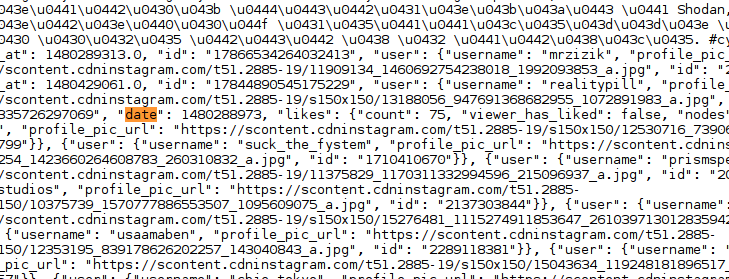
\includegraphics[width=120mm]{images/instagram/1.png}
	}
\end{figure}

It means, that I can simply get all data from specific web page even without any authorization. For parsing I used xpath and re library from python.

\begin{lstlisting}
script = html.xpath('//script[contains(., "window._sharedData")]/text()')[0]
data = re.search(r"window._sharedData = (.*?);\$", script).group(1)
data = json.loads(data)
\end{lstlisting}

All data was stored in \textbf{data} array.

\subsection{Finding range of instagram ip}
